%
% Explicación de redes Feistel, capítulo de antecedentes.
% Proyecto Lovelace.
%

\subsection{Redes Feistel}

Consiste en un \gls{gl:cifrado_iterativo} que mapea bloques de
texto en claro de tamaño $2t$bits (separados en bloques
$L_0, R_0$ de tamaño $t$) a un texto cifrado $R_r$, $L_r$
mediante un proceso de $r$ \glspl{gl:ronda}.

\begin{pseudocodigo}[caption={Feistel, cifrado.}, label={feistel:1}]
  inicio
  para_todo $i$ desde 1 hasta $r$:
    $L_i = R_{i-1}$
    $R_i = L_{i-1} \oplus f(R_{i-1}, K_i)$
  fin
  fin
\end{pseudocodigo}

Donde cada subllave $K_i$ se obtiene de la llave $K$.

Normalmente el número de rondas $r$ es mayor o igual a tres y par.
Además, casi siempre intercambia el orden de los bloques de salida al
revés en la última ronda: ($R_r, L_r$) en vez de ($L_r, R_r$).

El descifrado se realiza utilizando el mismo proceso de cifrado pero
con las llaves en el orden inverso (comenzando con $K_r$ hasta $K_1$).

\begin{figure}[H]
  \begin{center}
    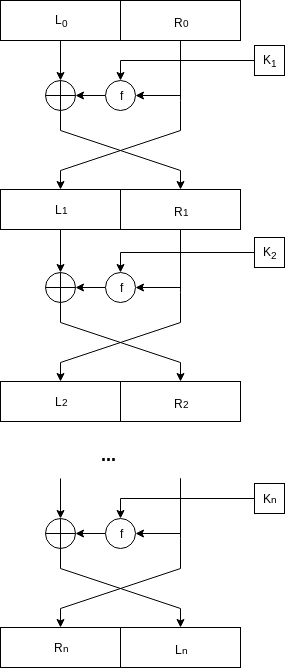
\includegraphics[width=0.25\linewidth]{diagramas/feistel}
     \caption{Diagrama genérico de una red Feistel.}
     \label{feistel}
   \end{center}
\end{figure}

Esta versión de las redes Feistel tiene como reestricción que la longitud
del bloque a procesar debe ser par. Existen dos generalizaciones del esquema
original que permiten procesar bloques de cualquier longitud: las redes Feistel
desbalanceadas y las redes Feistel alternantes (figura
\ref{feistel:generalizaciones})~\cite{sinopsis_rogaway}.

\subimport{/}{desbalanceadas}
\subimport{/}{alternantes}

\begin{figure}[H]
  \centering
  \begin{subfigure}{0.45\textwidth}
    \begin{center}
      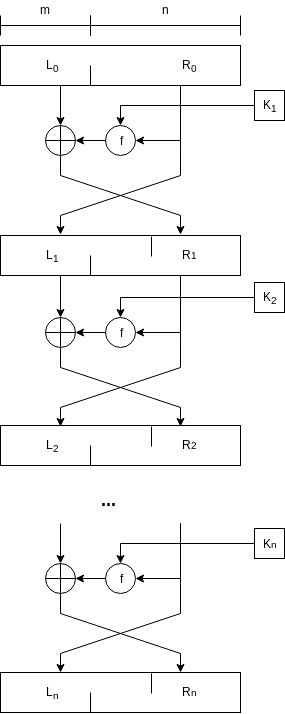
\includegraphics[width=0.5\linewidth]{diagramas/desbalanceadas.png}
      \caption{Redes desbalanceadas.}
      \label{feistel:desbalanceadas}
    \end{center}
  \end{subfigure}
  \begin{subfigure}{0.45\textwidth}
    \begin{center}
      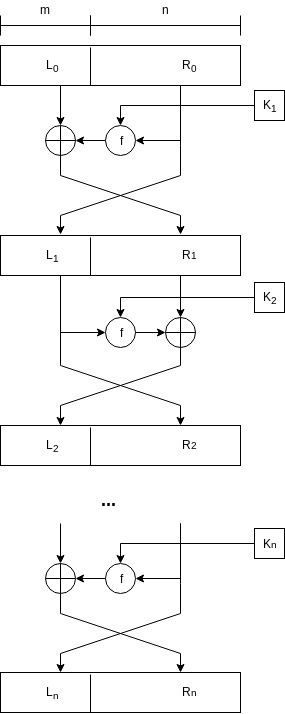
\includegraphics[width=0.5\linewidth]{diagramas/alternantes.png}
      \caption{Redes alternantes.}
      \label{feistel:alternantes}
    \end{center}
  \end{subfigure}
  \caption{Generalizaciones de las redes Feistel.}
  \label{feistel:generalizaciones}
\end{figure}
